\documentclass{csthesis-paper}

% 设置文档信息
\renewcommand{\stuname}{张三} % 学生姓名
\renewcommand{\stuid}{3210xxxxxx} % 学生学号
\renewcommand{\teaname}{李四} % 指导教师
\renewcommand{\stugrade}{2021级} % 学生年级
\renewcommand{\stumajor}{信息安全} % 学生专业
\renewcommand{\stucollege}{计算机科学与技术学院} % 学生所在学院
\renewcommand{\stutitle}{毕业设计题目} % 毕设题目
\renewcommand{\submitdate}{2025年5月12日} % 提交日期写系统提交日期即可
\renewcommand{\taskbegindate}{2024年6月13日} % 用于任务书的开始日期,一般是选导时间
\renewcommand{\taskenddate}{2025年5月30日} % 用于任务书的结束日期,一般是答辩时间
% 如果是涉密论文,取消下面这行的注释
% \SetSecretPaperTrue
% 如果不是涉密论文(默认),则无需任何操作,或者可以显式调用下面这行
% \SetSecretPaperFalse

\begin{document}
    % 封面
    \pagestyle{empty}

\AddToShipoutPictureBG*{
    \AtPageLowerLeft{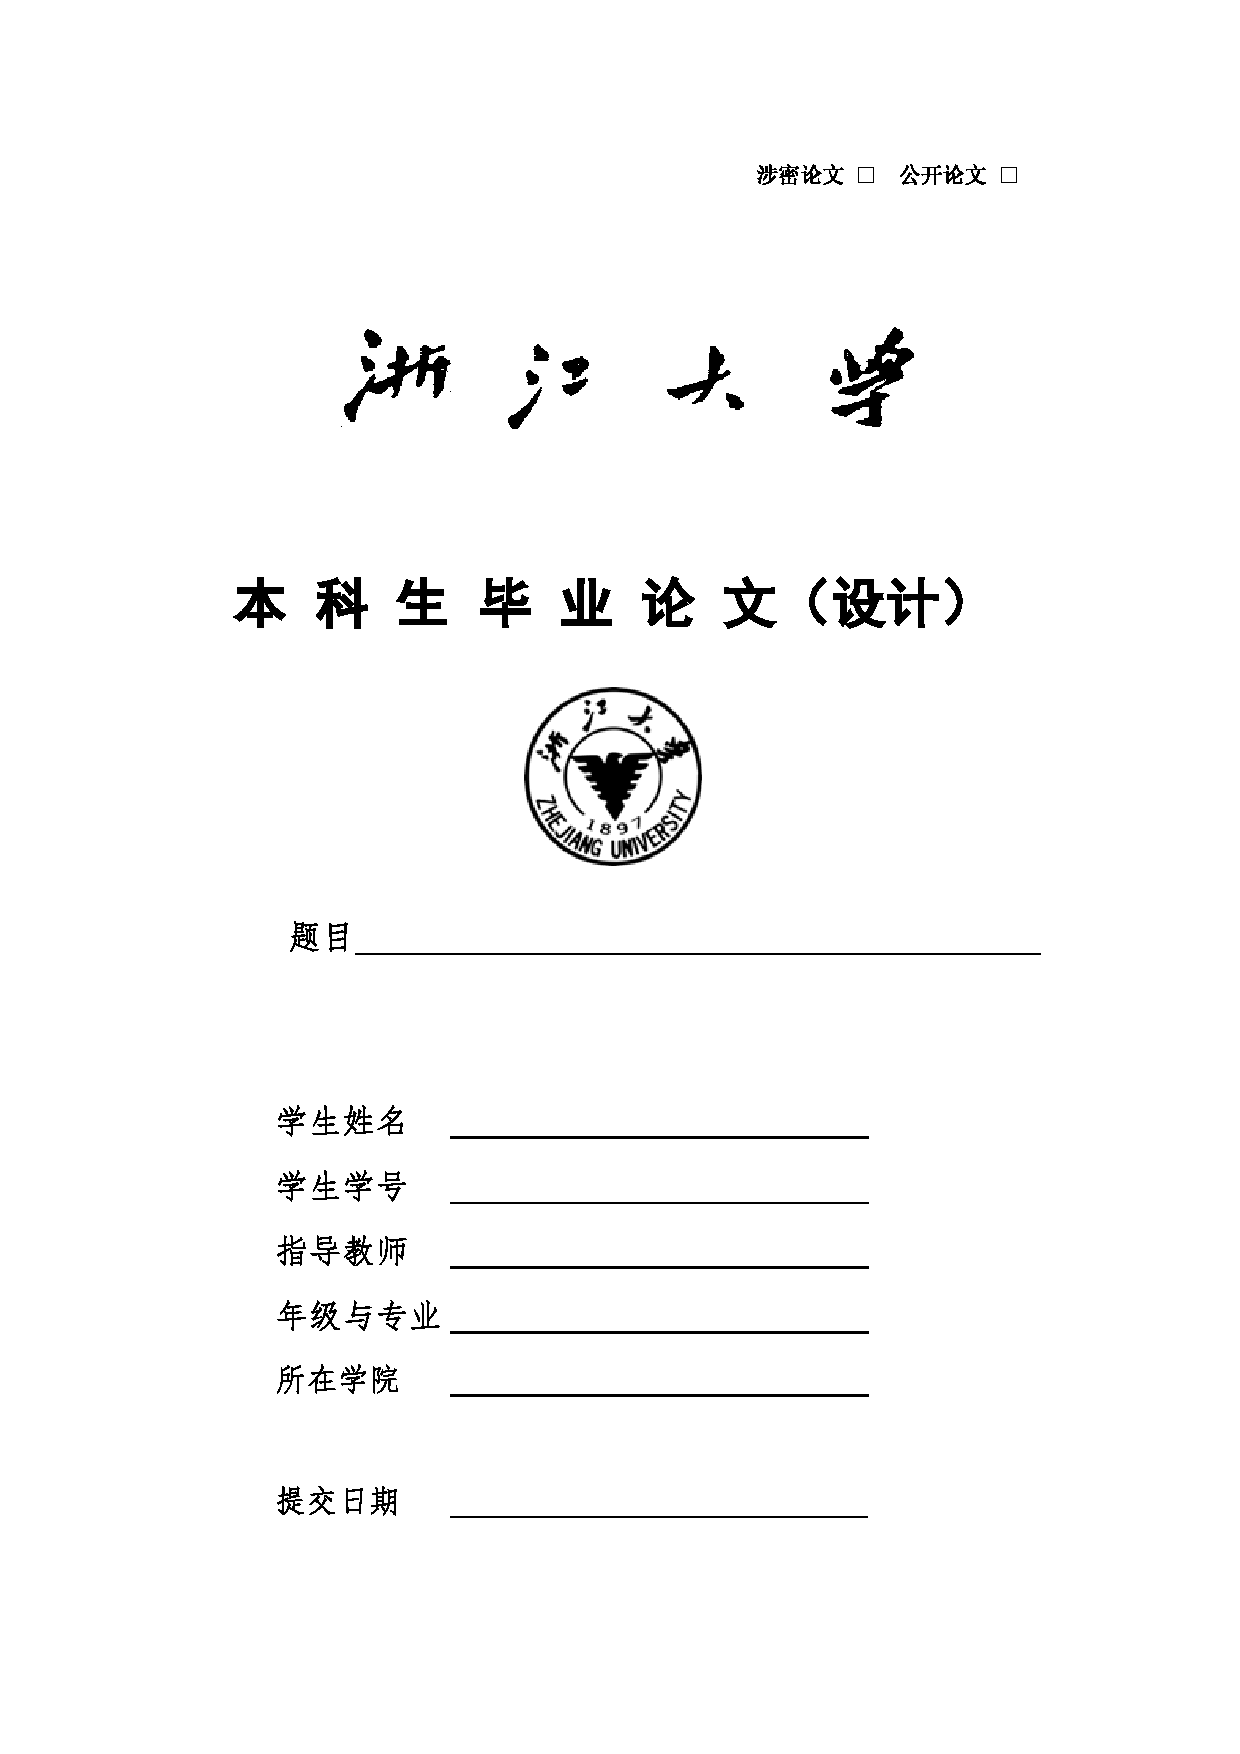
\includegraphics[width=\paperwidth,height=\paperheight]{pre-compiled-pdf/cover.pdf}}
}

\begin{textblock}{210}(49,153)
    \CJKfamily{fs}\zihao{3}\bfseries
    \setlength{\tabcolsep}{0pt}
    \newdimen\maxTitleHeight
    \settoheight{\maxTitleHeight}{\parbox{20em}{A\\A\\A}} % 题目的高度至多为三行
    \begin{tabular}{p{20em}} % 题目每行二十字,其余信息每行十二字
        \parbox[t][\maxTitleHeight][t]{20em}{\centering \stutitle} \\[3.6em]
        \hspace{2.8em} {\makebox[12em]{\stuname}} \\[0em]
        \hspace{2.8em} {\makebox[12em]{\stuid}} \\[-0.1em]
        \hspace{2.8em} {\makebox[12em]{\teaname}} \\[0em]
        \hspace{2.8em} {\makebox[12em]{\stugrade\hspace{0.6em}\stumajor}} \\[0em]
        \hspace{2.8em} {\makebox[12em]{\stucollege}} \\[1.6em]
        \hspace{2.8em} {\makebox[12em]{\submitdate}}
    \end{tabular}
\end{textblock}

\null\clearpage
    \pagestyle{Index}
    % 承诺书
    \cleardoublepage

\AddToShipoutPictureBG*{
    \AtPageLowerLeft{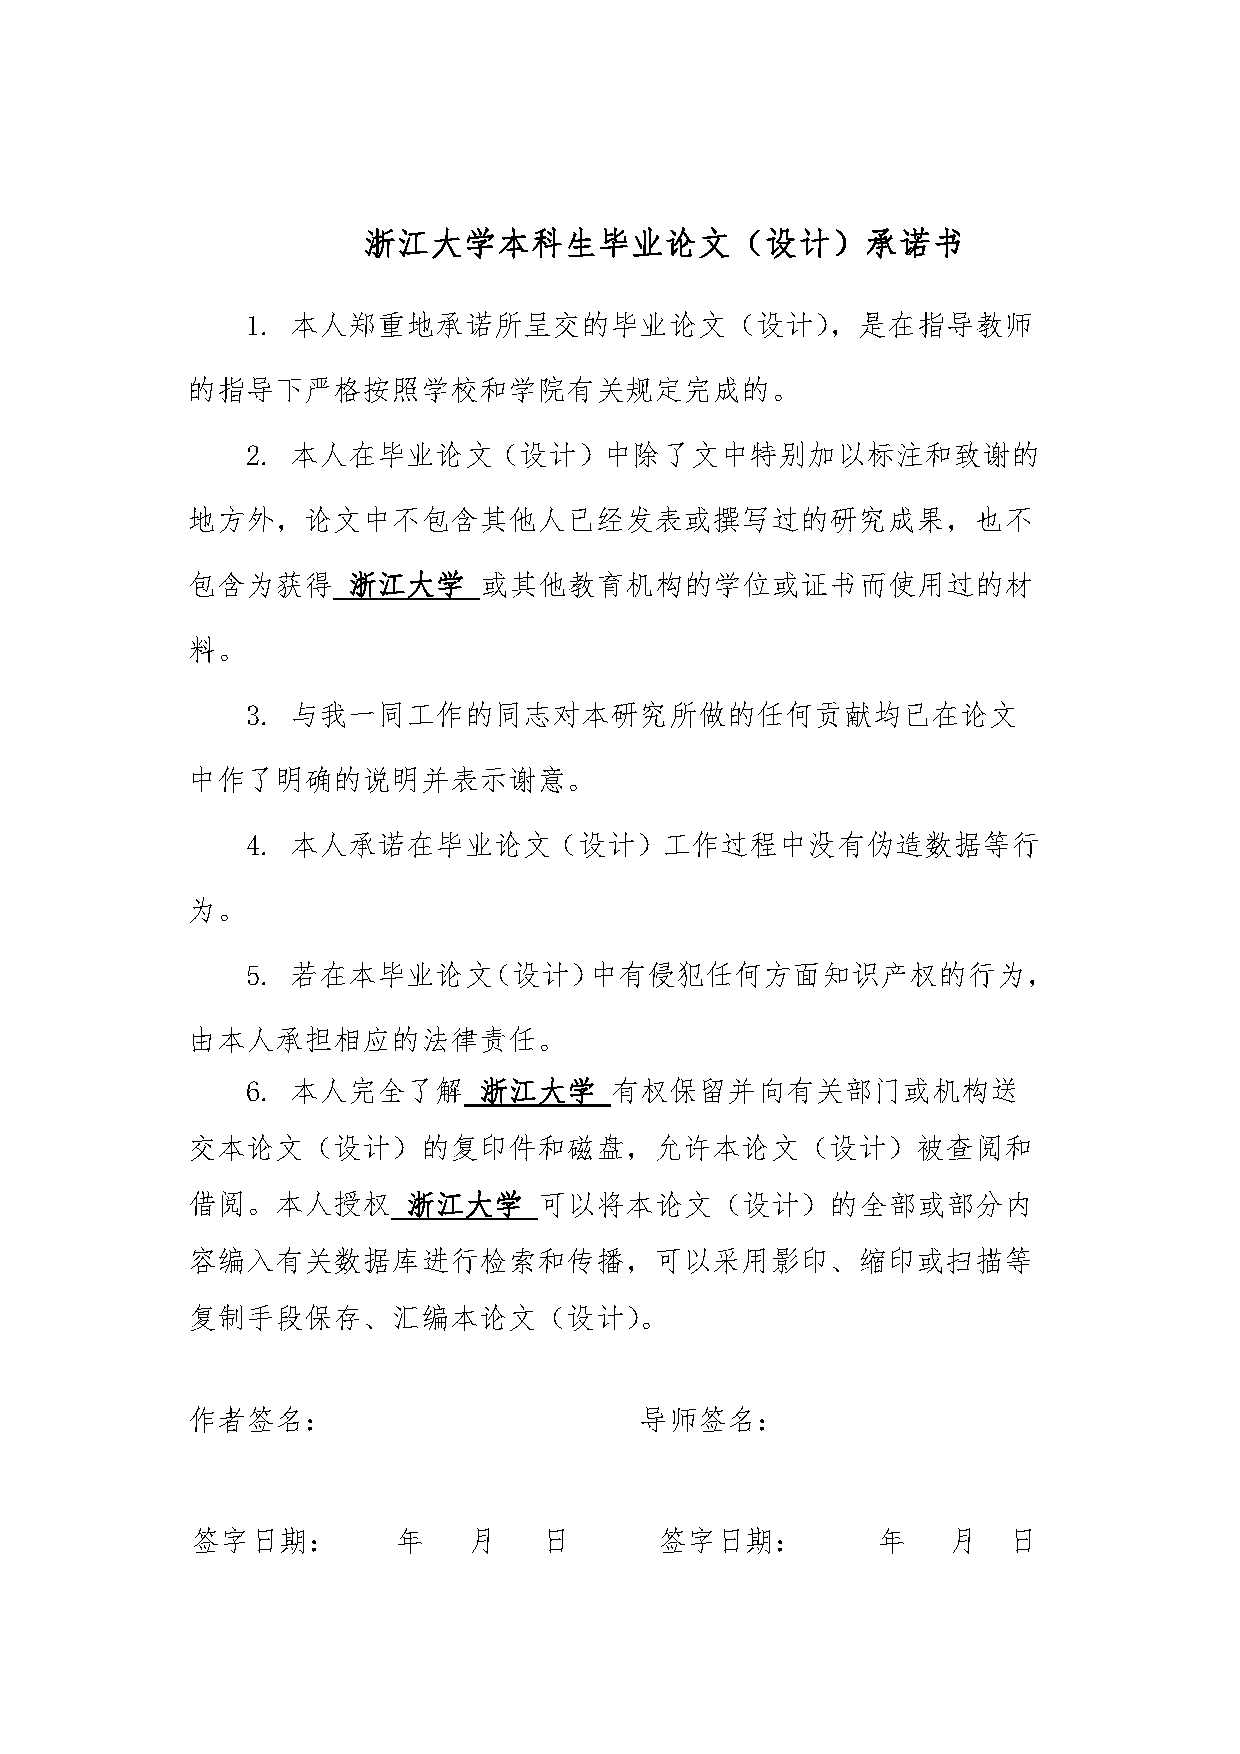
\includegraphics[width=\paperwidth,height=\paperheight]{pre-compiled-pdf/declaration.pdf}}
}

\null\clearpage
    % 致谢
    \cleardoublepage

\begin{center}
    ~\\[-1.5em]
    \zihao{3}\CJKfamily{fs}\textbf{致\quad 谢}
\end{center}

\zihao{-4}
% === 在这里填写致谢内容 ===

\par 感谢我的导师\teaname 教授在本课题研究过程中给予的悉心指导和帮助。
感谢我的同学们在课题研究过程中给予的支持和帮助。
感谢我的家人对我在课题研究过程中给予的支持和鼓励。
感谢学校提供的良好学习环境和资源支持。
感谢所有参与本课题研究的老师和同学们。
感谢所有为本课题研究提供帮助的人们。
    % 中英文摘要
    \cleardoublepage

\begin{center}
    ~\\[-1.5em]
    \zihao{3}\CJKfamily{fs}\textbf{摘\quad 要(中文)}
\end{center}

\zihao{-4}
% === 从此处开始填写中文摘要内容 ===
\par 《原神》是由米哈游自主研发的一款全新开放世界冒险游戏。
游戏发生在一个被称作「提瓦特」的幻想世界,在这里,被神选中的人将被授予「神之眼」,导引元素之力。
你将扮演一位名为「旅行者」的神秘角色,在自由的旅行中邂逅性格各异、能力独特的同伴们,和他们一起击败强敌。
% === 中文摘要内容结束 ===

\bigskip

% === 在这里填写中文关键词内容 ===
\noindent \textbf{关键词:}原神;开放世界;角色扮演;冒险游戏;米哈游
% === 中文关键词内容结束 ===
    \cleardoublepage

\begin{center}
    ~\\[-1.5em]
    \zihao{3}\CJKfamily{fs}\textbf{Abstract(英文)}
\end{center}

\zihao{-4}
% === 在这里填写英文摘要内容 ===
\par Genshin Impact is an open-world action RPG. In the game, set forth on a journey across a fantasy world 
called Teyvat. In this vast world, you can explore seven nations, meet a diverse cast of characters with 
unique personalities and abilities, and fight powerful enemies together with them, all on the way during 
your quest to find your lost sibling. You can also wander freely, immersing yourself in a world filled with 
life, and let your sense of wonder lead you to uncover all of its mysteries... Until you are at long last 
reunited with your lost sibling and bear witness to the culmination of all things at the end of your journey.
% === 英文摘要内容结束 ===

\bigskip

% === 在这里填写英文关键词内容 ===
\noindent \textbf{Keywords:} Genshin Impact; Open World; Role-playing Game; Adventure Game; miHoYo
% === 英文关键词内容结束 ===
    % 目录
    \cleardoublepage
\begin{center}
    ~\\[-1.5em]
    \zihao{3}\CJKfamily{fs}\textbf{目\quad 录}
\end{center}

\noindent \zihao{4}\CJKfamily{fs}\textbf{第一部分 \quad 毕业论文(设计)}
\vspace{-1em}
\tableofcontents

    % 文档主体部分
    \cleardoublepage
    \pagestyle{empty}
    \mypart{毕业论文(设计)}
    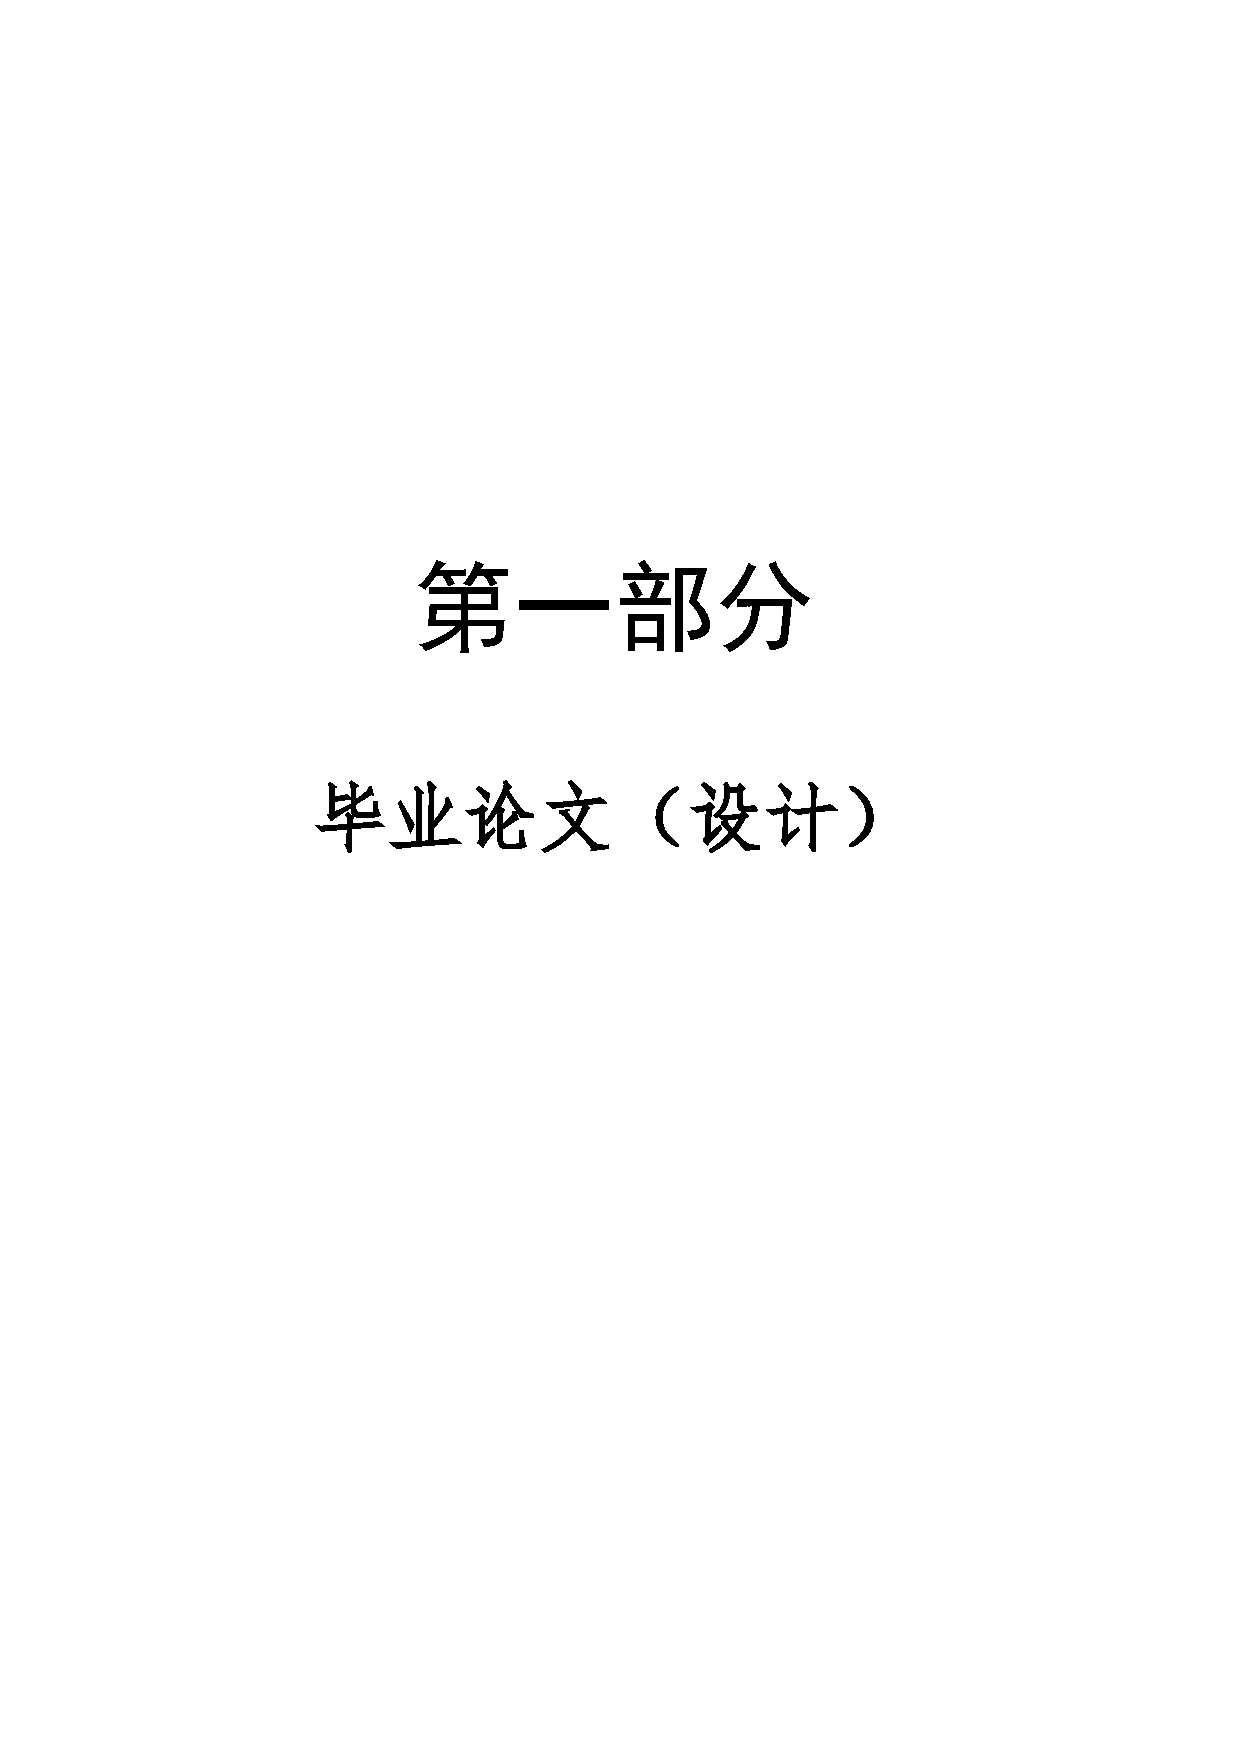
\includepdf[pages=1]{pre-compiled-pdf/big-part1.pdf}
    \cleardoublepage
    \pagestyle{Content}
    \zihao{-4}
    % \nocite{*} % 如果没有任何参考文献,需要手动添加一个空引用,这样 xe-bib-xe-xe 的编译链不会意外退出
% 正文部分,从这里开始

\section{绪论}

\subsection{背景}

\par 徐州地方,历代大规模征战五十余次,是非曲折难以论说,但史家无不注意到,正是在这个古战场,
决定了多少代王朝的盛衰兴亡、此兴彼落,所以古来就有问鼎中原之说。\upcite{schweizer2013comparative}

\subsection{节标题}

\section{章标题}

\subsection{节标题}

\subsubsection{小节标题}

\subsubsection{小节标题}

\newpage
\addNoindentTocEntry{参考文献}
\begin{center}
    ~\\[-1.5em]
    \zihao{3}\CJKfamily{fs}\textbf{参考文献}
\end{center}
\bibliographystyle{gbt7714-numerical}
\phantomsection		% 要想目录中参考文献的超链接正确需要加这一语句
{\normalfont\CJKfamily{Songti}\zihao{-4}\setlength{\baselineskip}{14pt}
\renewcommand{\refname}{\vspace{-\baselineskip}}
\bibliography{reference/thesis-refs}}
    % 附录,如果不需要附录,可以注释掉下面这一行
    \newpage
\addNoindentTocEntry{附录}
\begin{center}
    ~\\[-1.5em]
    \zihao{3}\CJKfamily{fs}\textbf{附\quad 录}
\end{center}

% === 以下内容仅作示例作用,实际内容请根据需要修改 ===

\setcounter{section}{1}
\renewcommand{\thesection}{A\arabic{section}}

\par 以下内容仅作示例作用,实际内容请根据需要修改。

\par \myeqref{equ:sample} 是一个示例公式。

\begin{equation}
  \label{equ:sample}
  A=\overbrace{(a+b+c)+\underbrace{i(d+e+f)}_{\text{虚数}}}^{\text{复数}}
\end{equation}

\par \myfigref{fig:sample} 是一个示例图片。

\begin{figure}[htbp]
  \centering
  \includegraphics[width=.3\linewidth]{images/zju-logo.jpg}
  \caption{\label{fig:sample}示例图片}
\end{figure}

\par \mytabref{tab:sample} 是一个示例表格。

\begin{table}[htbp]
  \caption{\label{tab:sample}自动调节列宽的表格}
  \begin{tabularx}{\linewidth}{c|X<{\centering}}
      \hline
      第一列 & 第二列 \\ \hline
      xxx & xxx \\ \hline
      xxx & xxx \\ \hline
      xxx & xxx \\ \hline
  \end{tabularx}
\end{table}

\par \myargref{alg:sample} 是一个算法样例。

\begin{algorithm}[H]
  \caption{算法样例}\label{alg:sample}
  \begin{algorithmic}[1] % [1] 参数表示行号从1开始
    \Require 数组 $A[low...high]$ 和起始索引 $low$,结束索引 $high$ % \Require 用于描述输入参数
    \Ensure 排序后的数组 $A$,其中元素按非递减顺序排列 % \Ensure 用于描述输出参数
    \Function{QuickSort}{$A, low, high$}
      \If{$low < high$}
        \State $pivot \gets$ \Call{Partition}{$A, low, high$} % \State 用于普通语句
        \State \Call{QuickSort}{$A, low, pivot-1$}
        \State \Call{QuickSort}{$A, pivot+1, high$}
      \EndIf
    \EndFunction
    
    \Statex
    
    \Function{Partition}{$A, low, high$}
      \State $pivot \gets A[high]$  \Comment{选择最后一个元素作为基准}
      \State $i \gets low-1$  \Comment{小于基准的元素的索引}
      \For{$j \gets low$ to $high-1$}
        \If{$A[j] \leq pivot$}
          \State $i \gets i+1$
          \State 交换 $A[i]$ 和 $A[j]$
        \EndIf
      \EndFor
      \State 交换 $A[i+1]$ 和 $A[high]$
      \State \Return $i+1$ % 返回结果
    \EndFunction
  \end{algorithmic}
\end{algorithm}
    % 作者简历
    \newpage
\addNoindentTocEntry{作者简历}

\begin{center}
    ~\\[-1.5em]
    \zihao{3}\CJKfamily{fs}\textbf{作者简历}
\end{center}

\zihao{-4}

\noindent 作者简历(示例)\\
\noindent 姓名:西西九八\quad 性别:女\quad 民族:汉\quad 出生年月:2003-02-26\quad 籍贯:浙江省杭州市 \\
\noindent 1992.09-1995.07\qquad 杭州市学军中学 \\
\noindent 1995.09-1999.07\qquad 浙江大学攻读学士学位 \\
\noindent 获奖情况:\\
\noindent 参加项目:\\
\noindent 发表的学术论文:\\

    % 任务书和考核表
    \pagestyle{empty}
    \cleardoublepage % 此页单面打印
\addNoindentTocEntry{《浙江大学本科生毕业论文(设计)任务书》}

\AddToShipoutPictureBG*{
    \AtPageLowerLeft{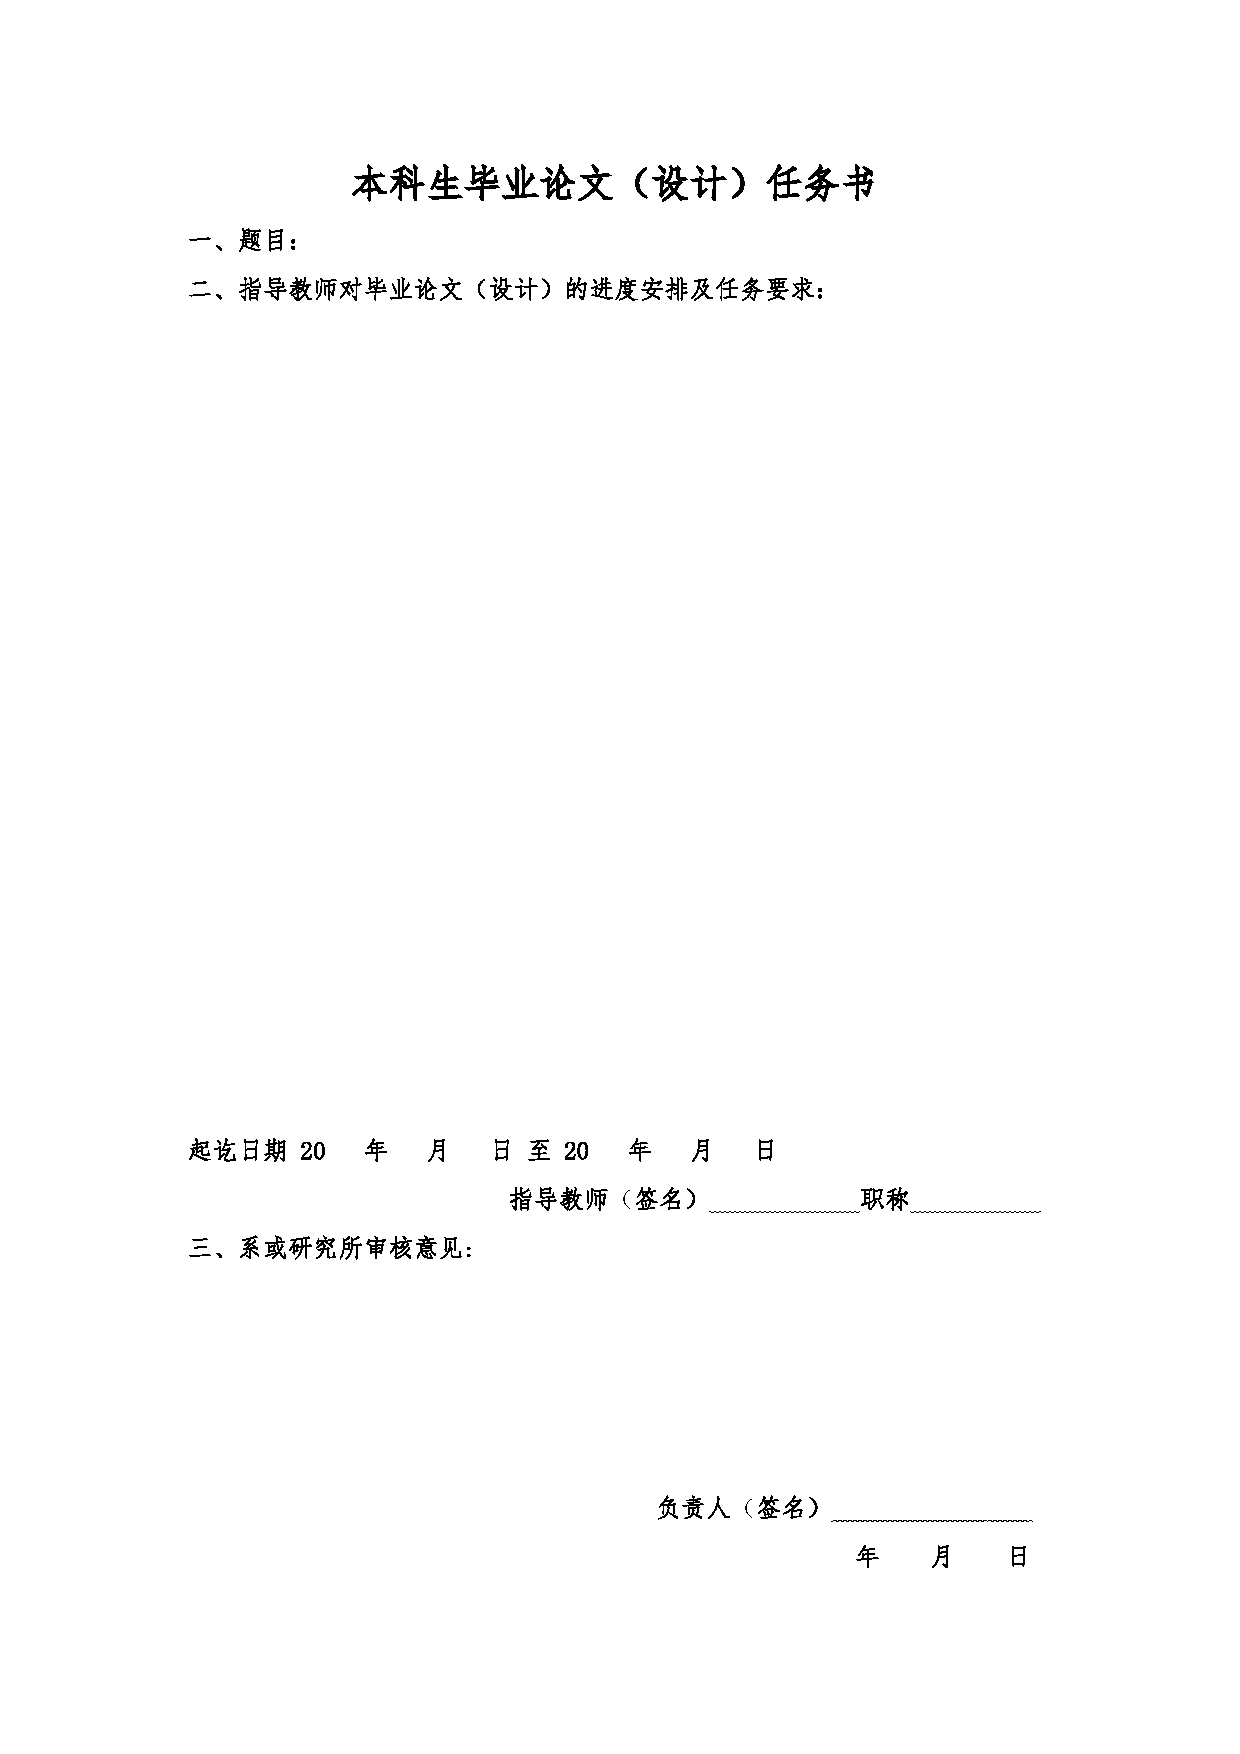
\includegraphics[width=\paperwidth,height=\paperheight]{pre-compiled-pdf/requirement.pdf}}
}

\begin{textblock}{210}(44.5,38.6)
    \CJKfamily{fs}\zihao{-4}\bfseries
    \makebox[28em][l]{\stutitle}
\end{textblock}

\begin{textblock}{210}(23.4,191.4)
    \CJKfamily{fs}\zihao{-4}\bfseries
    \makebox[28em][l]{起讫日期\hspace{0.5em}\taskbegindate\hspace{0.5em}至\hspace{0.5em}\taskenddate}
\end{textblock}

\begin{requirementtext}
    % === 在这里填写指导教师对毕业论文(设计)的进度安排及任务要求 ===
    \par 《原神》是由米哈游自主研发的一款全新开放世界冒险游戏。
    游戏发生在一个被称作「提瓦特」的幻想世界,在这里,被神选中的人将被授予「神之眼」,导引元素之力。
    你将扮演一位名为「旅行者」的神秘角色,在自由的旅行中邂逅性格各异、能力独特的同伴们,和他们一起击败强敌。
    % === 文本结束 ===
\end{requirementtext}

\null\clearpage
    \cleardoublepage % 此页单面打印
\addNoindentTocEntry{《浙江大学本科生毕业论文(设计)考核表》}

\AddToShipoutPictureBG*{
    \AtPageLowerLeft{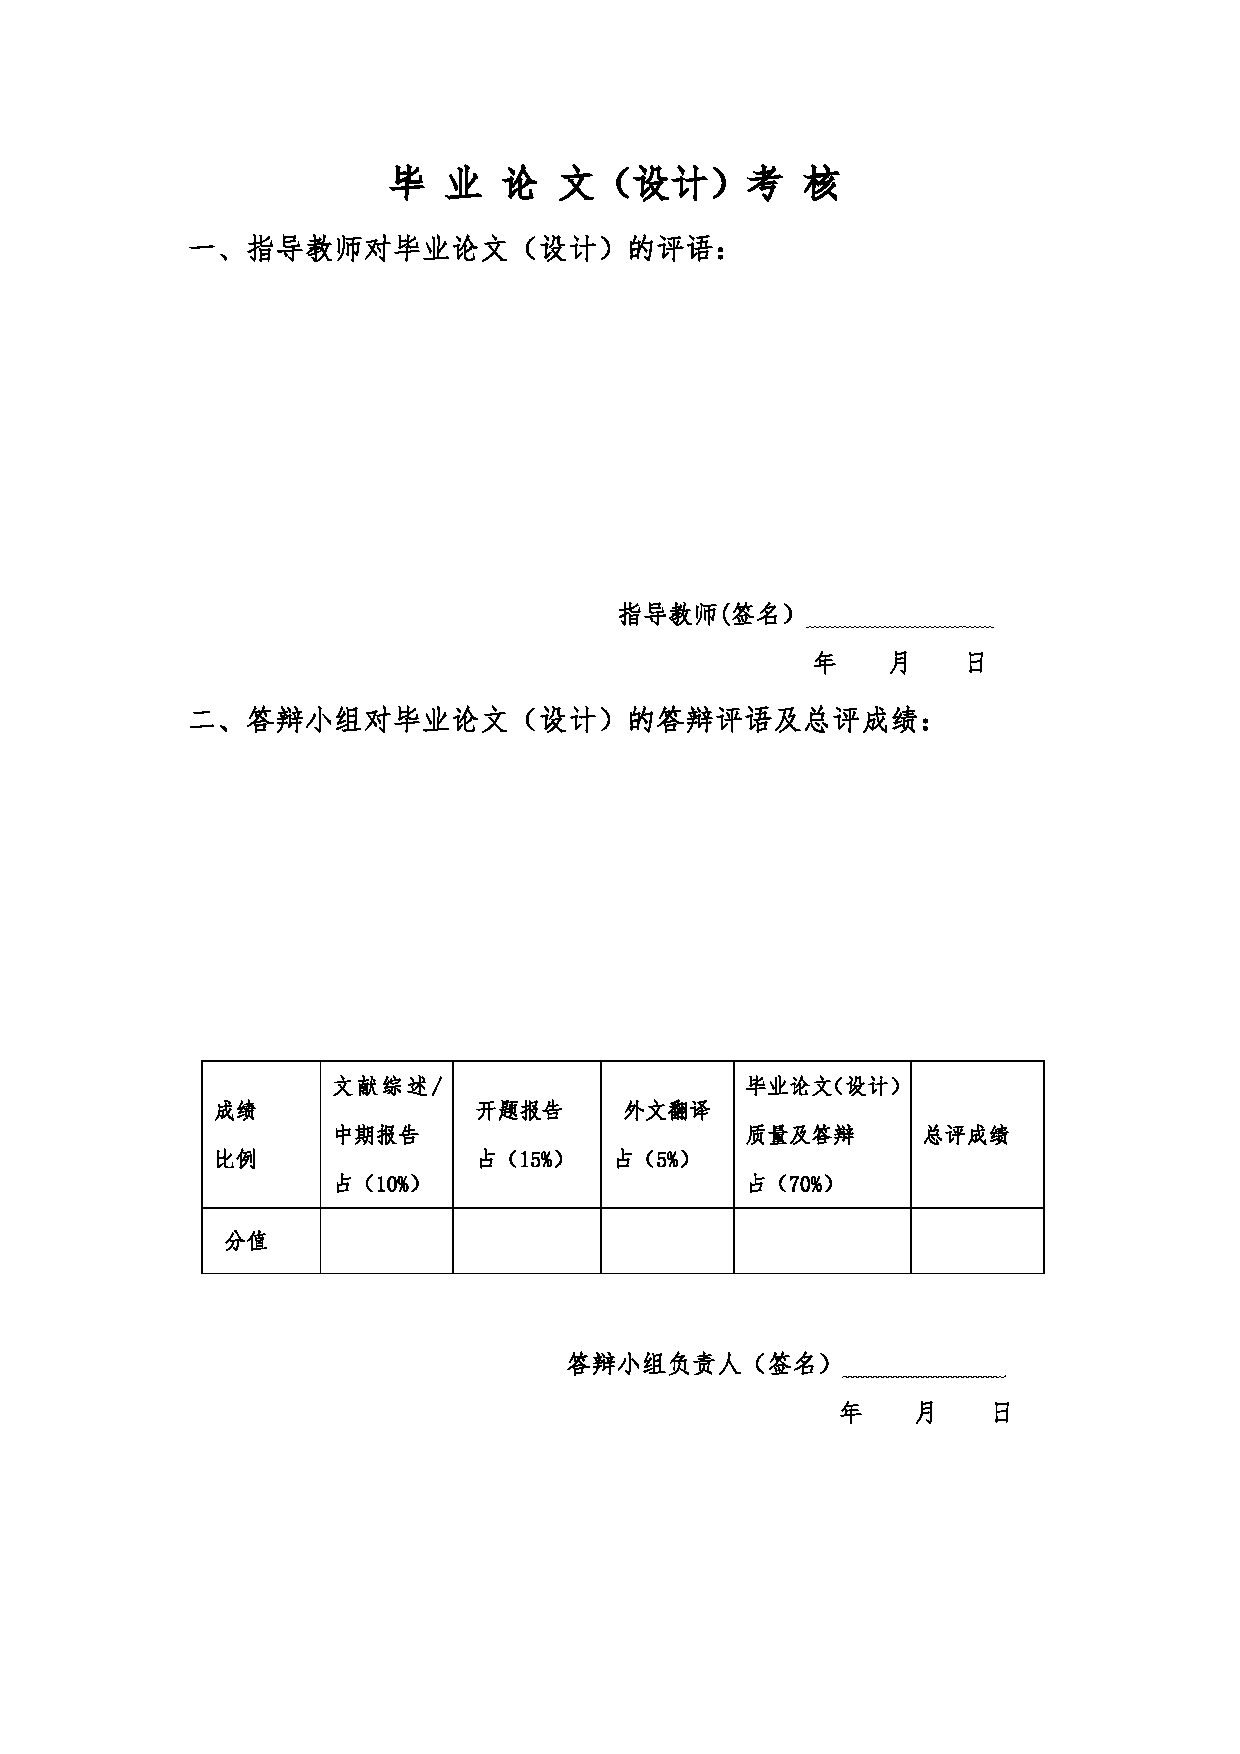
\includegraphics[width=\paperwidth,height=\paperheight]{pre-compiled-pdf/assessment.pdf}}
}

\begin{assessmenttext}
    % === 在这里填写指导教师对毕业论文(设计)的评语,评语从系统内导师评语复制 ===
    \par 《原神》是由米哈游自主研发的一款全新开放世界冒险游戏。
    游戏发生在一个被称作「提瓦特」的幻想世界,在这里,被神选中的人将被授予「神之眼」,导引元素之力。
    你将扮演一位名为「旅行者」的神秘角色,在自由的旅行中邂逅性格各异、能力独特的同伴们,和他们一起击败强敌。
    % === 指导教师对毕业论文(设计)的评语结束 ===
\end{assessmenttext}

\null\clearpage
    % 第二部分
    % \cleardoublepage
\pagestyle{empty}
\mypart{文献综述和开题报告}
% 手动向目录中添加目录条目
\addNoindentTocEntryWithPage{文献综述和开题报告封面}{-2} % 要求可以不编写页码,这里根据目录页的页码编写为 -2 页
\addNoindentTocEntryWithPage{指导教师对文献综述和开题报告具体内容要求}{-1} % 要求可以不编写页码,这里根据目录页的页码编写为 -1 页
\addNoindentTocEntryWithPageRoman{目录}{1} % 目录页页码固定为罗马数字 1
% === 以下的五条目录需要手动设置页码 ===
% 根据文献综述和开题报告的目录页的实际情况手动设置这里的页码,修改以下四条的第二个参数
\addNoindentTocEntryFsSectionWithPage{一、文献综述(中期报告)}{1}
\addNoindentTocEntryFsSectionWithPage{二、开题报告}{3}
\addNoindentTocEntryFsSectionWithPage{三、外文翻译}{5}
\addNoindentTocEntryFsSectionWithPage{四、外文原文}{7}
% 要求可以不编写页码,这里根据文献综述和开题报告的实际情况,编写为最后一页的页码加 1
\addNoindentTocEntryWithPage{《浙江大学本科生文献综述和开题报告考核表》}{8}
% ===                           ===
% 插入pdf文件
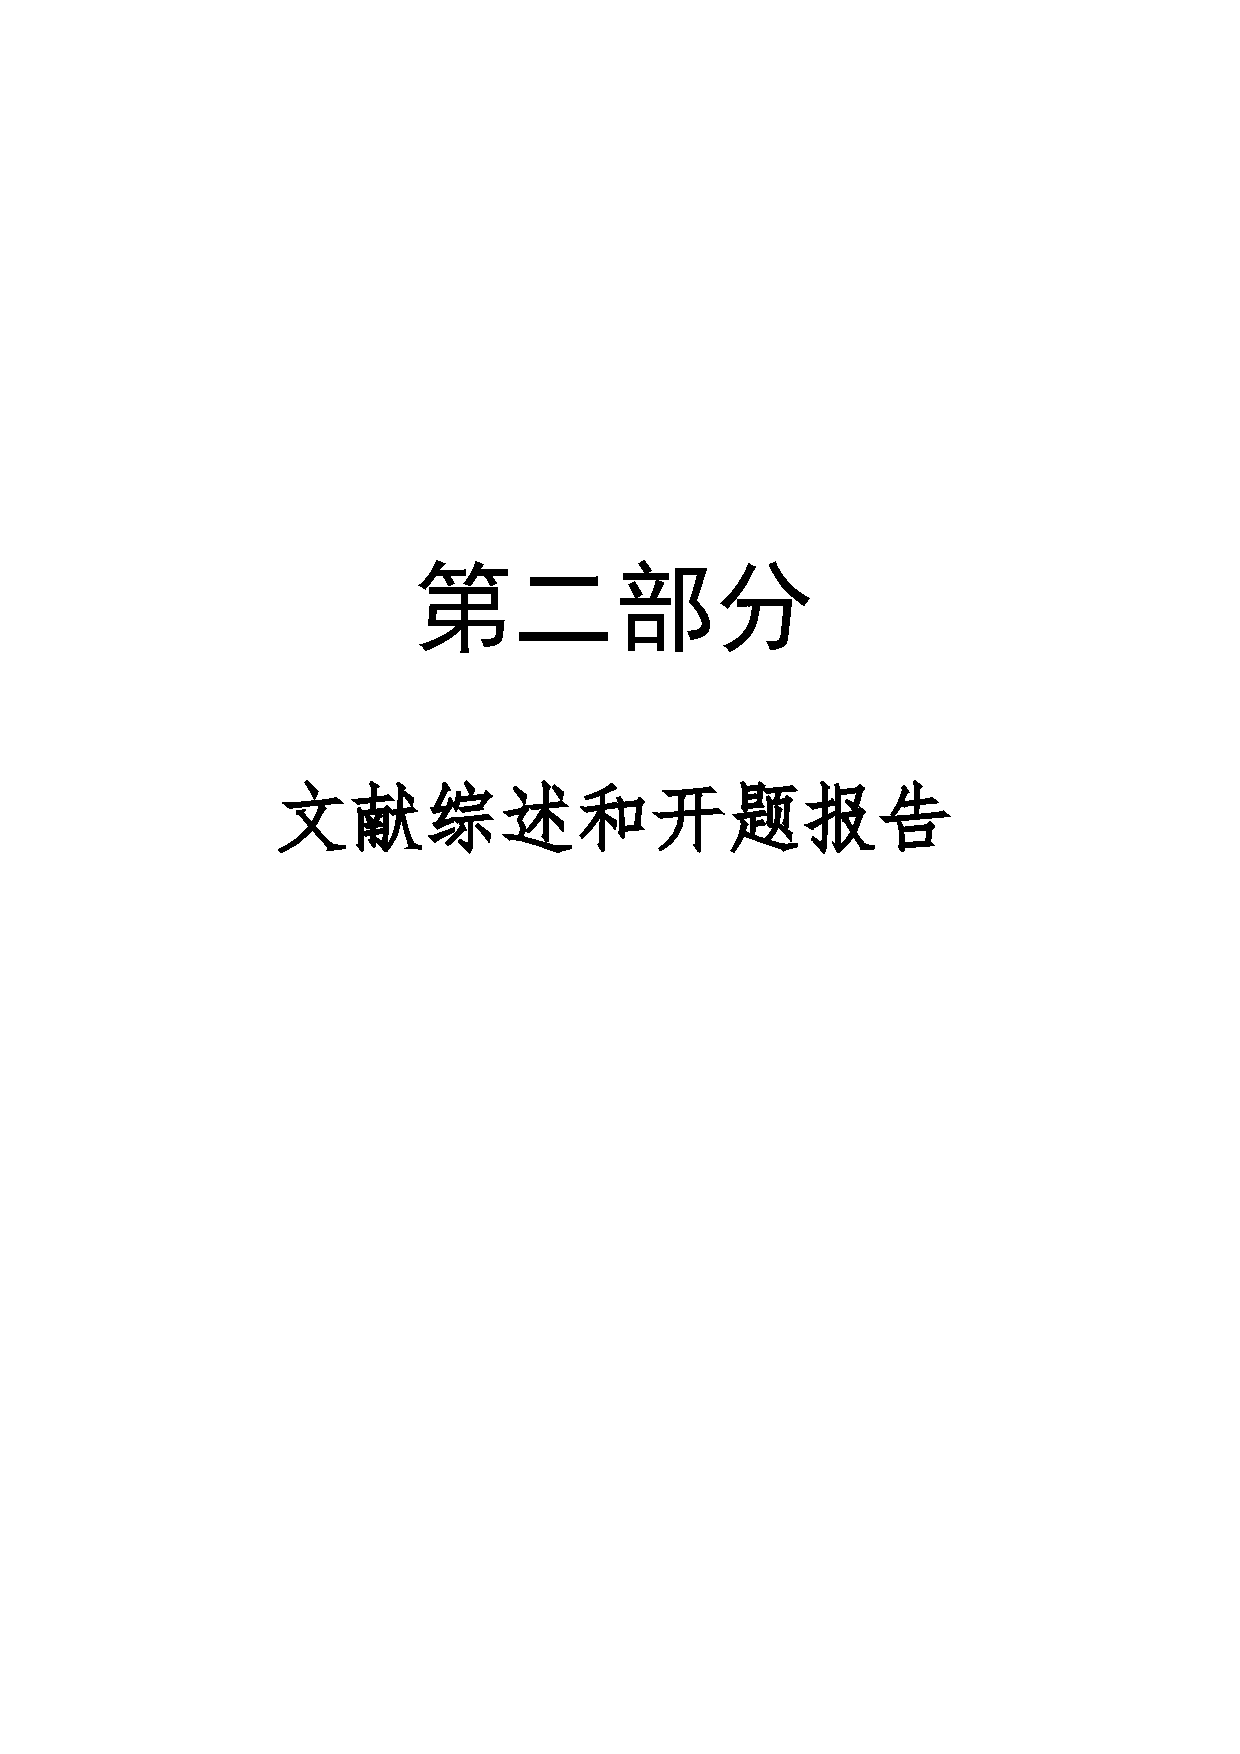
\includepdf[pages=1]{pre-compiled-pdf/big-part2.pdf}
\cleardoublepage
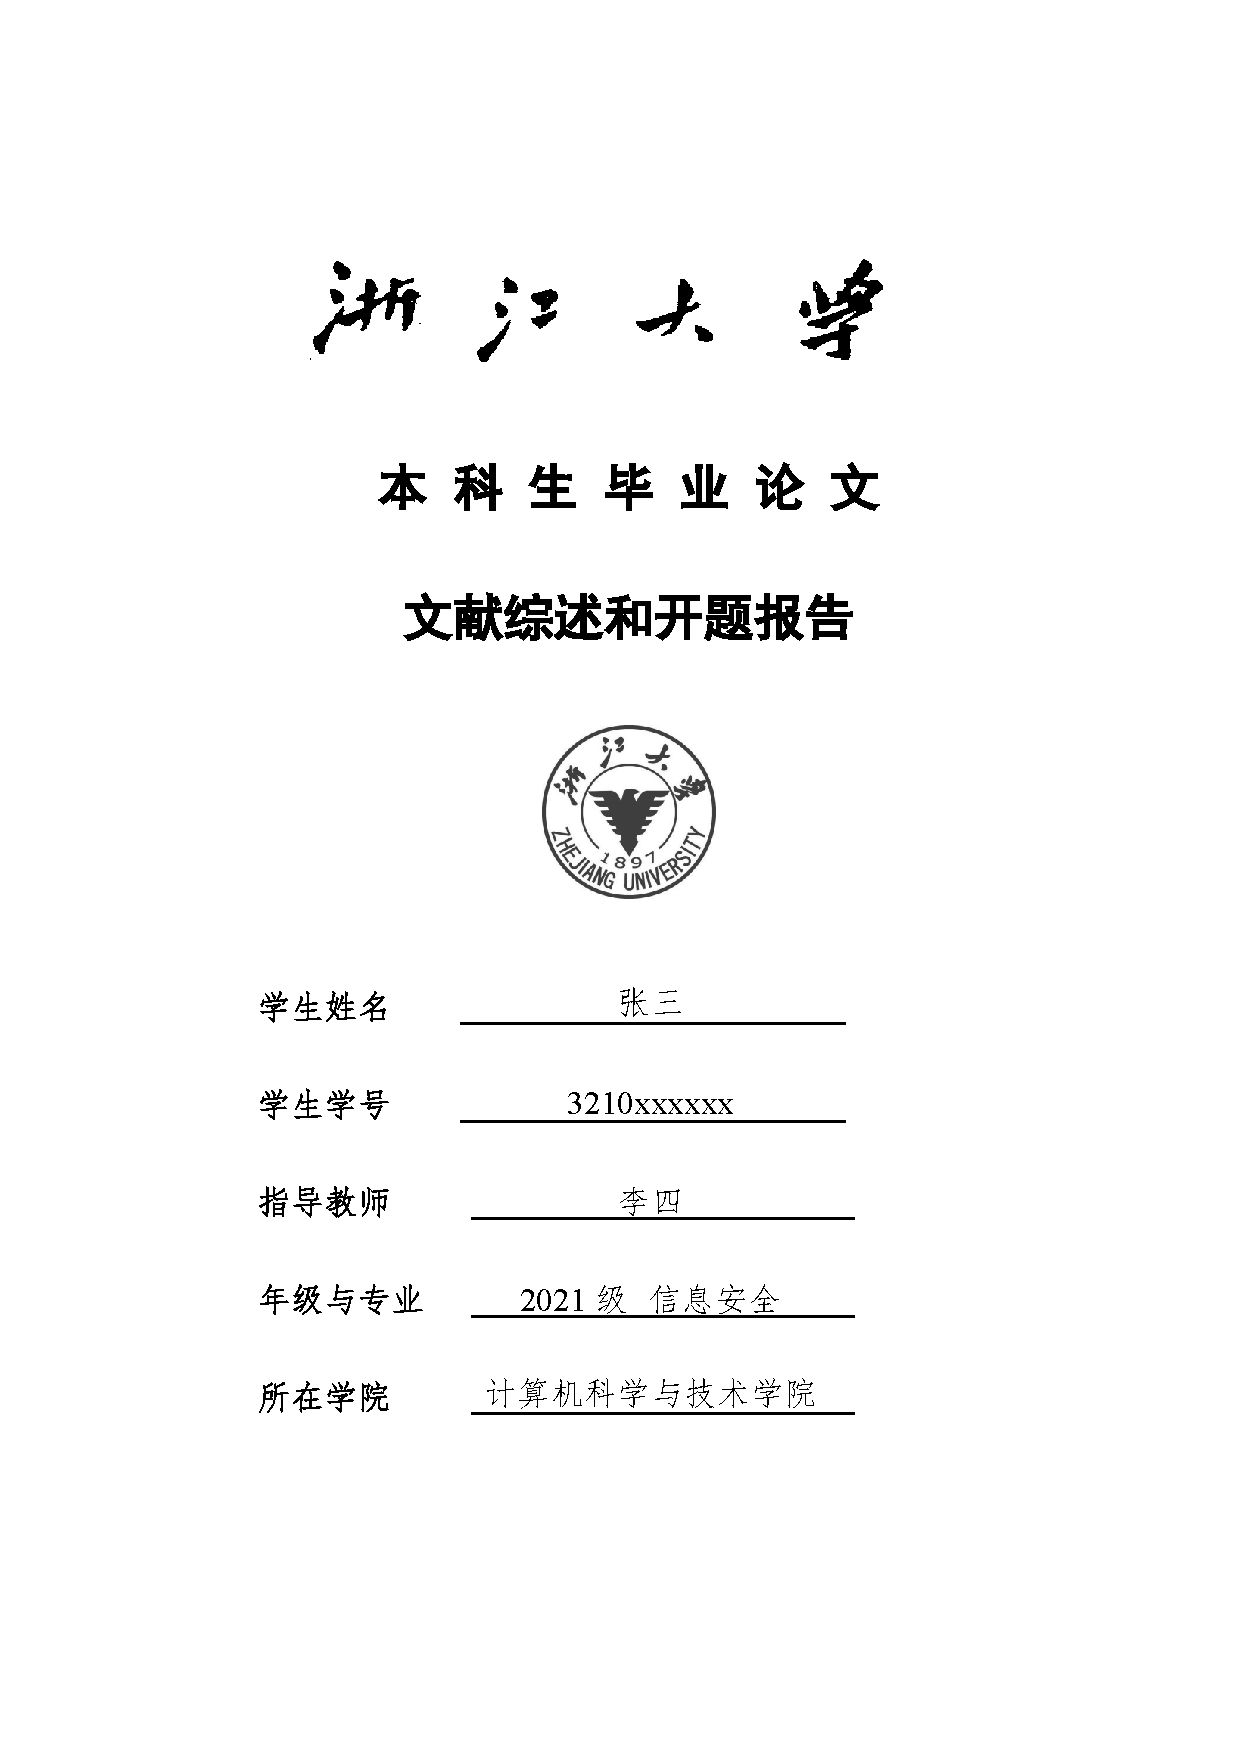
\includepdf[pages=1-,pagecommand={\pagestyle{Content}}]{mid/main.pdf}
\end{document}